\documentclass[12pt, twoside]{article}   	% use "amsart" instead of "article" for AMSLaTeX format
\usepackage{geometry}                		% See geometry.pdf to learn the layout options. There are lots.
\geometry{a4paper}                   		% ... or a4paper or a5paper or ... 
\linespread{1.0}
%\geometry{landscape}                		% Activate for rotated page geometry
%\usepackage[parfill]{parskip}    		% Activate to begin paragraphs with an empty line rather than an indent
\usepackage{graphicx}				% Use pdf, png, jpg, or eps§ with pdflatex; use eps in DVI mode
								% TeX will automatically convert eps --> pdf in pdflatex		

\pagestyle{headings}

%SetFonts

\usepackage{mathrsfs}
\usepackage{amsthm,amsmath,amssymb}

%\usepackage{fourier}
%\usepackage{newpxmath}
\usepackage{fontspec}
%\setmainfont{Scala}
%\setmonofont{SF Mono}
\usepackage{xeCJK}
\usepackage{bm}
\usepackage{bbold}

\def\rcurs{{\mbox{$\resizebox{.16in}{.08in}{\includegraphics{ScriptR}}$}}}
\def\brcurs{{\mbox{$\resizebox{.16in}{.08in}{\includegraphics{BoldR}}$}}}
\def\hrcurs{{\mbox{$\hat \brcurs$}}}

\usepackage{color,xcolor}
\usepackage{ebezier}
\usepackage{tikz}
%\usepackage{circuitikz}
\usepackage{physics}

\usepackage[colorlinks,
linkcolor = blue,
anchorcolor = blue,
citecolor = blue,
urlcolor = blue]{hyperref}

\usepackage{multirow}
\usepackage{multicol}
\usepackage{makecell}
\usepackage{wrapfig}
\usepackage{caption}

\usepackage{appendix}
\theoremstyle{plain}
\newtheorem{lemma}{Lemma}[section]
\newtheorem{theorem}[lemma]{Theorem}
\newtheorem{axiom}[lemma]{Axiom}
\newtheorem{corollary}[lemma]{Corollary}
\newtheorem{proposition}[lemma]{Proposition}
\theoremstyle{definition}
\newtheorem{definition}[lemma]{Definition}
\newtheorem{remark}{Remark}[section]
\newtheorem{example}[lemma]{Example}

\usepackage{syntonly}
%\syntaxonly

\title{Light Beat}
\author{黄远墨~~\textsf{2023141220092}}
\date{}							% Activate to display a given date or no date

\begin{document}
	% generates the title
	\maketitle
	
	Consider two light fields with field functions
	\begin{align}
		E_1(x, t) &= A_1 \cos\left( k_1 x - \omega_1 t \right) = A_1 \cos\left[ \omega_1 \left(
		x/c - t \right) \right], \\
		E_2(x, t) &= A_2 \cos\left( k_2 x - \omega_2 t \right) = A_2 \cos\left[ \omega_2 \left(
		x/c - t \right) \right].
	\end{align}
	Total field
	\begin{equation}
		\begin{aligned}
			E(x, t) =& E_1(x, t) + E_2(x, t) = \frac{A_1 + A_2}{2} \Big[ \cos\left( \omega_1
			(x/c - t) \right) + \cos\left( \omega_2 (x/c - t) \right)\Big]\\
					&\phantom{000000000}+ \frac{A_1 - A_2}{2} \Big[ \cos\left( \omega_1
					(x/c - t) \right)
					- \cos\left( \omega_2 (x/c - t) \right) \Big]\\
					=& (A_1 + A_2) \cos\left[ \Omega (x/c - t)
					\right] \cos\left[ \omega (x/c - t) \right]\\
					 &- (A_1 - A_2) \sin\left[ \Omega (x/c - t)
					 \right] \sin\left[ \omega (x/c - t) \right],
		\end{aligned}
	\end{equation}
	where $\Omega = (\omega_1 - \omega_2) / 2$ and $\omega = (\omega_1 + \omega_2) / 2$.

	For large $\omega_1 + \omega_2 \gg \abs{\omega_1 - \omega_2}$, we can approximately see the total
	field as the composition of two rapidly oscillating field with slowly varying amplitudes:
	\begin{equation}
		E(x, t) = \mathcal A_1(x, t) \cos\omega(x/c - t) + \mathcal A_2(x, t) \sin\omega(x/c - t).
	\end{equation}
	Therefore, the intensity
	\begin{equation}
		\begin{aligned}
			I(x, t) = \abs{E(x, t)}^2 &\leq \abs{\mathcal A_1(x, t)}^2 + \abs{\mathcal A_2(x, t)}^2\\
									  &= A_1^2 + A_2^2 + 2 A_1 A_2 \cos 2\Omega(x/c - t).
		\end{aligned}
	\end{equation}
	That is, the enclosure of $I(x, t)$ is
	\begin{equation}
		I_{\text{enc}}(x, t) = A_1^2 + A_2^2 + 2 A_1 A_2 \cos(\omega_1 - \omega_2) (x/c - t).
	\end{equation}
	The wavelength of the enclosure $\lambda = \frac{2 \pi}{\omega_1 - \omega_2}$ is much larger
	than the wavelengths of two original light fields.
	
	An instance is demonstrated on the next page.

	\begin{figure}[htbp]
		\centering
		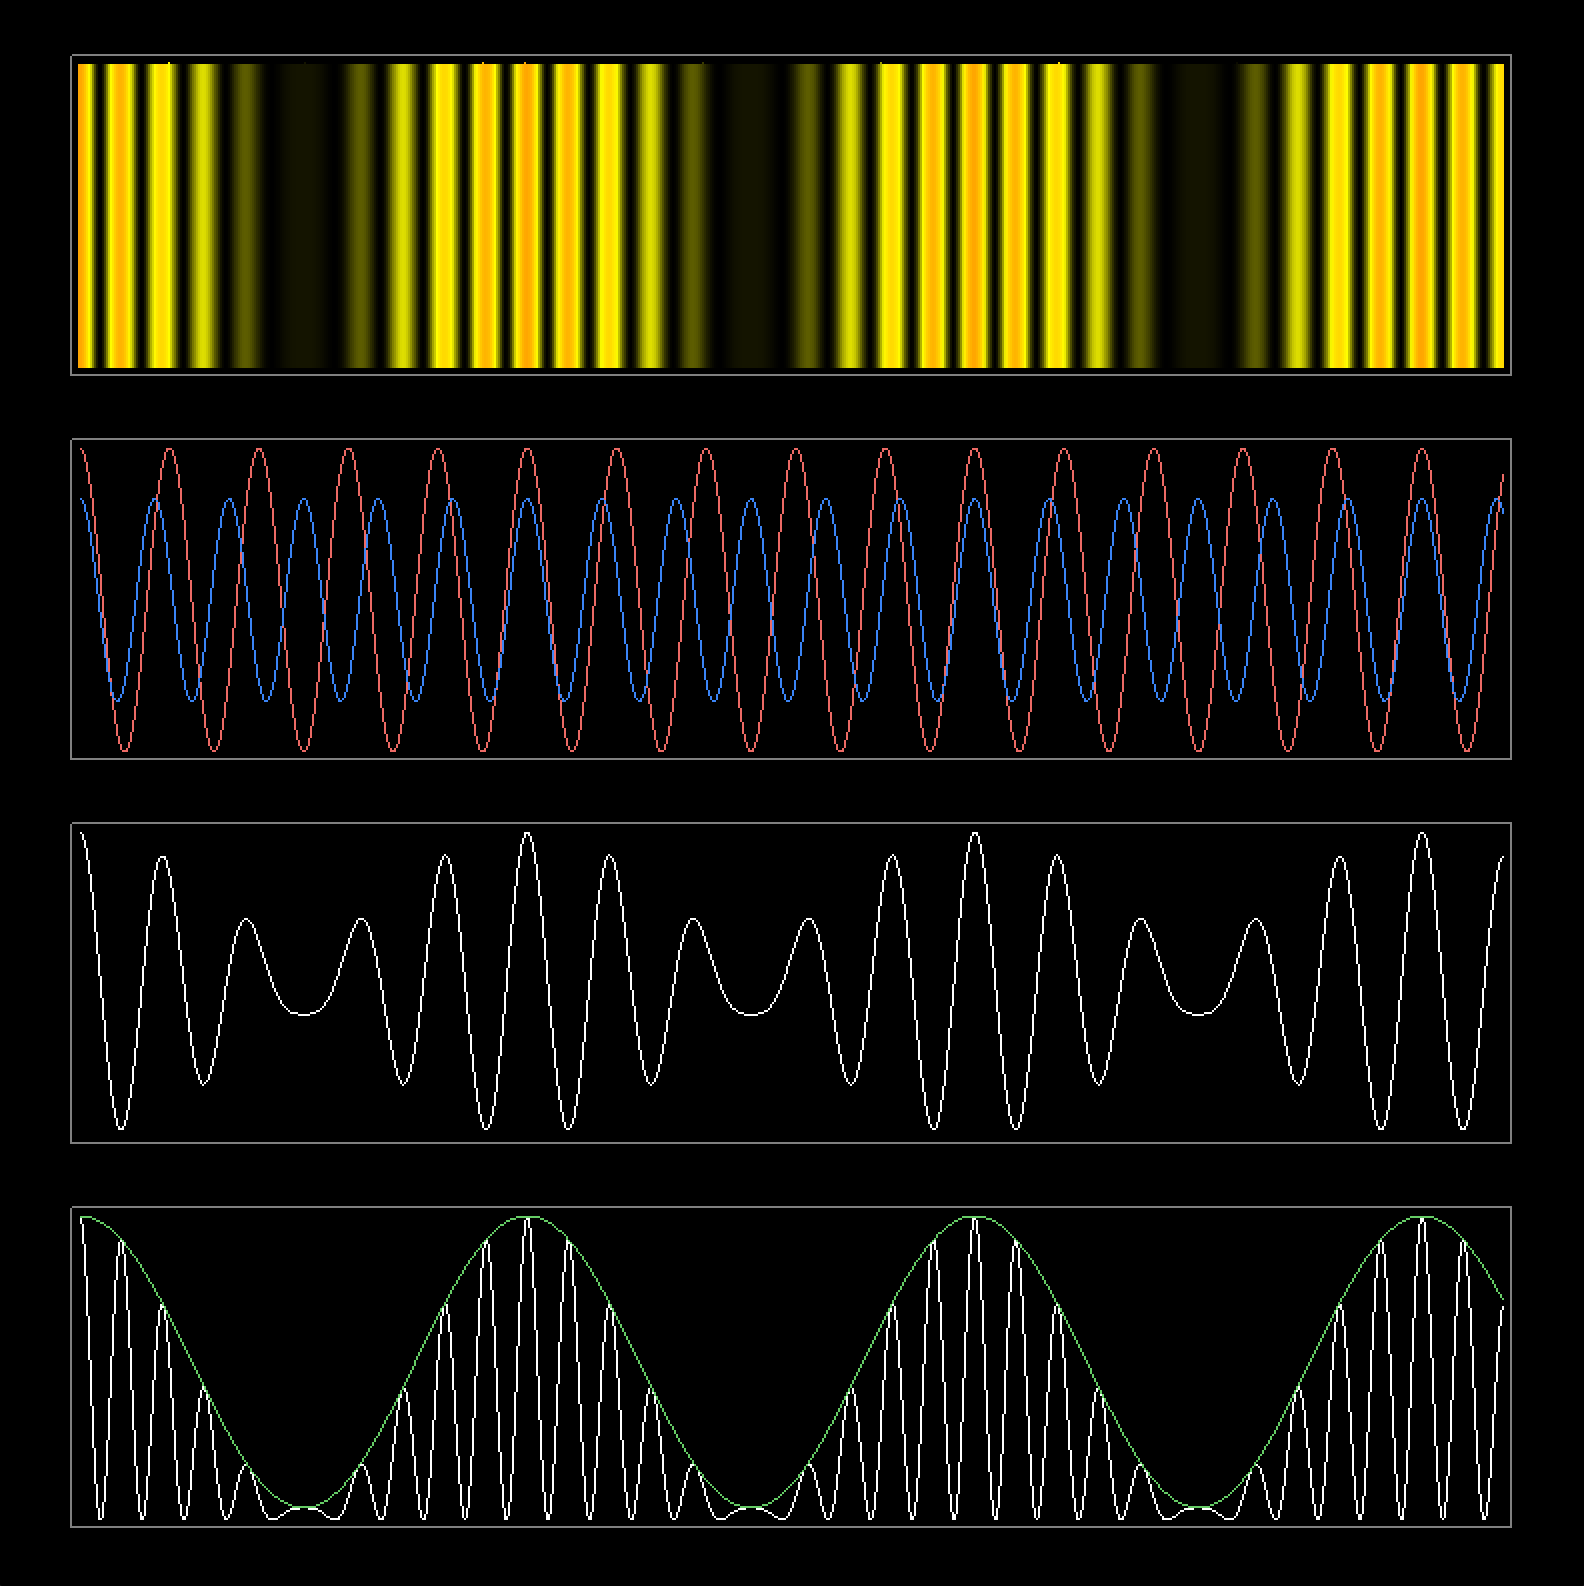
\includegraphics[width=\linewidth]{LightBeat}
		\captionsetup{font={small}}
		\caption{In this series of figures, we have taken $A_1 / A_2 = 1.5$, $\omega_2 / \omega_1
		= 1.2$. $x$ axis (space) is horizontal and $t = 0$. \\ The first figure is the simulated
		light intensity. \\ The second figure is the original two light fields. \\ The third figure
		is the total light field. \\ The last figure is the total light intensity with enclosure
		(the green curve).}
	\end{figure}
	
	
\end{document}


